\ifnum\pdfoutput=0
  \def\pgfsysdriver{pgfsys-dvisvgm.def}
\fi
\documentclass[tikz,border=0pt]{standalone}
\usepackage{tikz}
\usetikzlibrary{arrows.meta,calc}
\usepackage{amsmath,amssymb}
\usepackage{mlmodern}

% Colors matching blog _variables.scss and academic dark theme
\definecolor{bg}{HTML}{1E1E1E}
\definecolor{treeline}{HTML}{BEBEBE}
\definecolor{mutedline}{HTML}{5A5A5A}
\definecolor{gridline}{HTML}{4A4A4A}
\definecolor{digitcolor}{HTML}{E2E2E2}
\definecolor{neutralfill}{HTML}{B0B0B0}

% Distinct basis highlight colors for E_0, E_1, E_2, E_3
\definecolor{colE0}{HTML}{19D4FA}
\definecolor{colE1}{HTML}{4CE0B3}
\definecolor{colE2}{HTML}{F7B955}
\definecolor{colE3}{HTML}{F27289}

% Closed rectangle macro using -- cycle so dvisvgm emits single-M SVG paths
\newcommand{\drawrect}[5]{
    \draw[#1] (#2, #3) -- (#4, #3) -- (#4, #5) -- (#2, #5) -- cycle;
}

% Typeset \Big)^{#1} with the exact vertical height and depth of \Big( so left and right parentheses align identically
% (Uses raw TeX \setbox/\hbox instead of LaTeX \sbox so dvisvgm does not inject a black color group reset)
\newcommand{\rparenpow}[1]{%
    \begingroup
    \setbox0=\hbox{$\Big($}%
    \setbox2=\hbox{$\Big)^{\!#1}$}%
    \ht2=\ht0
    \dp2=\dp0
    \box2%
    \endgroup
}

% Helper macro to draw a matrix of total size \Msize centered at (#1, #2)
% #1 = cx, #2 = cy, #3 = N (1, 2, 4, 8), #4 = comma-separated r/c of 1-cells, #5 = fill color, #6 = border color, #7 = border lw
\newcommand{\drawmat}[7]{
    \pgfmathsetmacro{\xL}{#1 - 0.5*\Msize}
    \pgfmathsetmacro{\yB}{#2 - 0.5*\Msize}
    \pgfmathsetmacro{\xR}{#1 + 0.5*\Msize}
    \pgfmathsetmacro{\yT}{#2 + 0.5*\Msize}
    \pgfmathsetmacro{\cellw}{\Msize / #3}

    % Background of matrix
    \fill[bg] (\xL, \yB) rectangle (\xR, \yT);

    % Filled 1-cells
    \foreach \r/\c in {#4} {
        \pgfmathsetmacro{\cxL}{\xL + \c * \cellw}
        \pgfmathsetmacro{\cyT}{\yT - \r * \cellw}
        \pgfmathsetmacro{\cyB}{\cyT - \cellw}
        \pgfmathsetmacro{\cxR}{\cxL + \cellw}
        \fill[#5] (\cxL, \cyB) rectangle (\cxR, \cyT);
    }

    % Internal grid lines (if N > 1)
    \ifnum#3>1
        \pgfmathsetmacro{\NmOne}{#3 - 1}
        \foreach \k in {1,...,\NmOne} {
            \pgfmathsetmacro{\gx}{\xL + \k * \cellw}
            \pgfmathsetmacro{\gy}{\yB + \k * \cellw}
            \draw[gridline, line width=0.55pt] (\gx, \yB) -- (\gx, \yT);
            \draw[gridline, line width=0.55pt] (\xL, \gy) -- (\xR, \gy);
        }
    \fi

    % Outer border
    \drawrect{#6, line width=#7, line join=miter}{\xL}{\yB}{\xR}{\yT}
}

% Helper macro to draw a companion matrix \alpha of total size \Msize centered at (#1, #2)
% #1 = cx, #2 = cy, #3 = N (2, 4, 8), #4 = lower-left \beta 1-cells, #5 = \beta fill color, #6 = I_n 1-cells, #7 = border color, #8 = border lw
\newcommand{\drawalphamat}[8]{
    \pgfmathsetmacro{\xL}{#1 - 0.5*\Msize}
    \pgfmathsetmacro{\yB}{#2 - 0.5*\Msize}
    \pgfmathsetmacro{\xR}{#1 + 0.5*\Msize}
    \pgfmathsetmacro{\yT}{#2 + 0.5*\Msize}
    \pgfmathsetmacro{\cellw}{\Msize / #3}

    % Background of matrix
    \fill[bg] (\xL, \yB) rectangle (\xR, \yT);

    % Lower-left quadrant (\beta) 1-cells in the basis color
    \foreach \r/\c in {#4} {
        \pgfmathsetmacro{\cxL}{\xL + \c * \cellw}
        \pgfmathsetmacro{\cyT}{\yT - \r * \cellw}
        \pgfmathsetmacro{\cyB}{\cyT - \cellw}
        \pgfmathsetmacro{\cxR}{\cxL + \cellw}
        \fill[#5] (\cxL, \cyB) rectangle (\cxR, \cyT);
    }

    % Top-right and bottom-right (I_n) 1-cells in neutralfill
    \foreach \r/\c in {#6} {
        \pgfmathsetmacro{\cxL}{\xL + \c * \cellw}
        \pgfmathsetmacro{\cyT}{\yT - \r * \cellw}
        \pgfmathsetmacro{\cyB}{\cyT - \cellw}
        \pgfmathsetmacro{\cxR}{\cxL + \cellw}
        \fill[neutralfill] (\cxL, \cyB) rectangle (\cxR, \cyT);
    }

    % Internal grid lines
    \pgfmathsetmacro{\NmOne}{#3 - 1}
    \foreach \k in {1,...,\NmOne} {
        \pgfmathsetmacro{\gx}{\xL + \k * \cellw}
        \pgfmathsetmacro{\gy}{\yB + \k * \cellw}
        \draw[gridline, line width=0.55pt] (\gx, \yB) -- (\gx, \yT);
        \draw[gridline, line width=0.55pt] (\xL, \gy) -- (\xR, \gy);
    }

    % Outer border
    \drawrect{#7, line width=#8, line join=miter}{\xL}{\yB}{\xR}{\yT}

    % Border around the lower-left quadrant (\beta) in the basis color
    \drawrect{#5, line width=#8, line join=miter}{\xL}{\yB}{#1}{#2}
}

\begin{document}
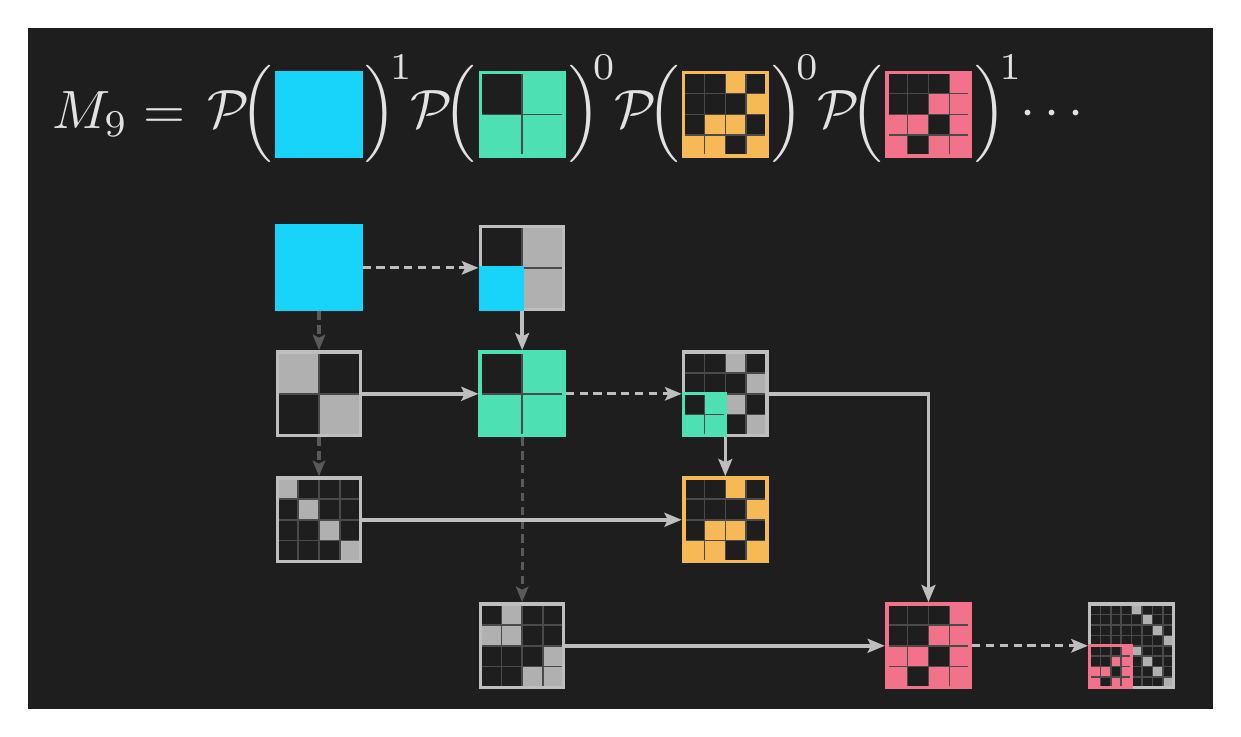
\begin{tikzpicture}[x=1cm, y=1cm]
    % Total width: 15.05, height: 8.65 (x from -1.25 to 13.80)
    \path[use as bounding box] (-1.25, -0.35) rectangle (13.80, 8.30);
    \fill[bg] (-1.25, -0.35) rectangle (13.80, 8.30);

    % Shared matrix visual size (all matrices 1x1, 2x2, 4x4, 8x8 have equal area!)
    \def\Msize{1.06}
    % Half of the outer border stroke width (1.4pt / 2 = 0.7pt = 0.0246cm) so arrow tips land flush on the outer edge
    \def\bpad{0.024}

    % Evenly spaced column x-centers (spacing = 2.58)
    \def\xZero{2.45}
    \def\xOne{5.03}
    \def\xTwo{7.61}
    \def\xThree{10.19}
    \def\xFour{12.77}

    % Row y-centers
    \def\yTop{7.20}
    \def\yRzero{5.25}
    \def\yRone{3.65}
    \def\yRtwo{2.05}
    \def\yRthree{0.45}

    % Arrow styles
    \tikzset{
        flowarrow/.style={
            treeline,
            line width=1.25pt,
            line join=miter,
            -{Stealth[length=6.2pt, width=5.0pt, inset=1.2pt]}
        },
        alphaarrow/.style={
            treeline,
            line width=1.20pt,
            densely dashed,
            line join=miter,
            -{Stealth[length=6.0pt, width=4.8pt, inset=1.2pt]}
        },
        embedarrow/.style={
            mutedline,
            line width=1.15pt,
            densely dashed,
            line join=miter,
            -{Stealth[length=5.6pt, width=4.5pt, inset=1.1pt]}
        }
    }

    % =========================================================================
    % TOP EQUATION ROW: M_9 = P(E_0)^1 P(E_1)^0 P(E_2)^0 P(E_3)^1 ...
    % =========================================================================

    % "M_9 =" on the left
    \node[color=digitcolor, scale=1.95, anchor=east, inner sep=0pt] at ({\xZero - 0.5*\Msize - 1.15}, \yTop) {$M_9 =$};

    % P( E_0 )^1 centered with E_0 at \xZero
    \node[color=digitcolor, scale=1.95, anchor=east, inner sep=0pt] at ({\xZero - 0.5*\Msize - 0.04}, \yTop) {$\mathcal{P}\!\Big($};
    \drawmat{\xZero}{\yTop}{1}{0/0}{colE0}{colE0}{1.35pt}
    \node[color=digitcolor, scale=1.95, anchor=west, inner sep=0pt] at ({\xZero + 0.5*\Msize + 0.04}, \yTop) {\rparenpow{1}};

    % P( E_1 )^0 centered with E_1 at \xOne
    \node[color=digitcolor, scale=1.95, anchor=east, inner sep=0pt] at ({\xOne - 0.5*\Msize - 0.04}, \yTop) {$\mathcal{P}\!\Big($};
    \drawmat{\xOne}{\yTop}{2}{0/1, 1/0, 1/1}{colE1}{colE1}{1.35pt}
    \node[color=digitcolor, scale=1.95, anchor=west, inner sep=0pt] at ({\xOne + 0.5*\Msize + 0.04}, \yTop) {\rparenpow{0}};

    % P( E_2 )^0 centered with E_2 at \xTwo
    \node[color=digitcolor, scale=1.95, anchor=east, inner sep=0pt] at ({\xTwo - 0.5*\Msize - 0.04}, \yTop) {$\mathcal{P}\!\Big($};
    \drawmat{\xTwo}{\yTop}{4}{0/2, 1/3, 2/1, 2/2, 3/0, 3/1, 3/3}{colE2}{colE2}{1.35pt}
    \node[color=digitcolor, scale=1.95, anchor=west, inner sep=0pt] at ({\xTwo + 0.5*\Msize + 0.04}, \yTop) {\rparenpow{0}};

    % P( E_3 )^1 centered with E_3 at \xThree
    \node[color=digitcolor, scale=1.95, anchor=east, inner sep=0pt] at ({\xThree - 0.5*\Msize - 0.04}, \yTop) {$\mathcal{P}\!\Big($};
    \drawmat{\xThree}{\yTop}{4}{0/3, 1/2, 1/3, 2/0, 2/1, 2/3, 3/0, 3/2, 3/3}{colE3}{colE3}{1.35pt}
    \node[color=digitcolor, scale=1.95, anchor=west, inner sep=0pt] at ({\xThree + 0.5*\Msize + 0.04}, \yTop) {\rparenpow{1}};

    % Trailing ellipsis "..."
    \node[color=digitcolor, scale=1.95, anchor=west, inner sep=0pt] at ({\xThree + 0.5*\Msize + 0.62}, \yTop) {$\cdots$};

    % =========================================================================
    % DASHED VERTICAL EMBEDDING ARROWS (drawn BEFORE matrices so tails sit cleanly underneath)
    % =========================================================================

    % E_0 -> E'_0 (vertical down in column 0)
    \draw[embedarrow] (\xZero, {\yRzero - 0.5*\Msize - \bpad}) -- (\xZero, {\yRone + 0.5*\Msize + \bpad});

    % E'_0 -> E''_0 (vertical down in column 0)
    \draw[embedarrow] (\xZero, {\yRone - 0.5*\Msize - \bpad}) -- (\xZero, {\yRtwo + 0.5*\Msize + \bpad});

    % E_1 -> E'_1 (vertical down in column 1)
    \draw[embedarrow] (\xOne, {\yRone - 0.5*\Msize - \bpad}) -- (\xOne, {\yRthree + 0.5*\Msize + \bpad});

    % =========================================================================
    % ORTHOGONAL MULTIPLICATION ARROWS (drawn BEFORE matrices so tails sit cleanly underneath)
    % =========================================================================

    % 1. E_0 -> alpha_1 (horizontal alpha-embedding)
    \draw[alphaarrow] ({\xZero + 0.5*\Msize + \bpad}, \yRzero) -- ({\xOne - 0.5*\Msize - \bpad}, \yRzero);

    % 2. E'_0 -> E_1 (horizontal) and alpha_1 -> E_1 (vertical down)
    \draw[flowarrow] ({\xZero + 0.5*\Msize}, \yRone) -- ({\xOne - 0.5*\Msize - \bpad}, \yRone);
    \draw[flowarrow] (\xOne, {\yRzero - 0.5*\Msize}) -- (\xOne, {\yRone + 0.5*\Msize + \bpad});

    % 3. E_1 -> alpha_2 (horizontal alpha-embedding)
    \draw[alphaarrow] ({\xOne + 0.5*\Msize + \bpad}, \yRone) -- ({\xTwo - 0.5*\Msize - \bpad}, \yRone);

    % 4. E''_0 -> E_2 (horizontal across column 1)
    \draw[flowarrow] ({\xZero + 0.5*\Msize}, \yRtwo) -- ({\xTwo - 0.5*\Msize - \bpad}, \yRtwo);

    % 5. alpha_2 -> E_2 (vertical down)
    \draw[flowarrow] (\xTwo, {\yRone - 0.5*\Msize}) -- (\xTwo, {\yRtwo + 0.5*\Msize + \bpad});

    % 6. alpha_2 -> E_3 (right from center of right edge of alpha_2, then straight down to top center of E_3)
    \draw[flowarrow] ({\xTwo + 0.5*\Msize}, \yRone) -- (\xThree, \yRone) -- (\xThree, {\yRthree + 0.5*\Msize + \bpad});

    % 7. E'_1 -> E_3 (horizontal across column 2)
    \draw[flowarrow] ({\xOne + 0.5*\Msize}, \yRthree) -- ({\xThree - 0.5*\Msize - \bpad}, \yRthree);

    % 8. E_3 -> alpha_3 (horizontal alpha-embedding)
    \draw[alphaarrow] ({\xThree + 0.5*\Msize + \bpad}, \yRthree) -- ({\xFour - 0.5*\Msize - \bpad}, \yRthree);

    % =========================================================================
    % LOWER GRID OF MATRICES (drawn ON TOP of arrow tails)
    % =========================================================================

    % --- Row 0 (y = \yRzero): E_0 (1x1) and alpha_1 (2x2) ---
    % E_0 (1x1) at (\xZero, \yRzero)
    \drawmat{\xZero}{\yRzero}{1}{0/0}{colE0}{colE0}{1.4pt}

    % alpha_1 (2x2) at (\xOne, \yRzero) with lower-left \beta = E_0 in colE0
    \drawalphamat{\xOne}{\yRzero}{2}{1/0}{colE0}{0/1, 1/1}{treeline}{1.15pt}

    % --- Row 1 (y = \yRone): E'_0 (2x2), E_1 (2x2), alpha_2 (4x4) ---
    % E'_0 (2x2) = I_2 at (\xZero, \yRone)
    \drawmat{\xZero}{\yRone}{2}{0/0, 1/1}{neutralfill}{treeline}{1.15pt}

    % E_1 (2x2) at (\xOne, \yRone)
    \drawmat{\xOne}{\yRone}{2}{0/1, 1/0, 1/1}{colE1}{colE1}{1.4pt}

    % alpha_2 (4x4) at (\xTwo, \yRone) with lower-left \beta = E_1 in colE1
    \drawalphamat{\xTwo}{\yRone}{4}{2/1, 3/0, 3/1}{colE1}{0/2, 1/3, 2/2, 3/3}{treeline}{1.15pt}

    % --- Row 2 (y = \yRtwo): E''_0 (4x4) and E_2 (4x4) ---
    % E''_0 (4x4) = I_4 at (\xZero, \yRtwo)
    \drawmat{\xZero}{\yRtwo}{4}{0/0, 1/1, 2/2, 3/3}{neutralfill}{treeline}{1.15pt}

    % E_2 (4x4) at (\xTwo, \yRtwo)
    \drawmat{\xTwo}{\yRtwo}{4}{0/2, 1/3, 2/1, 2/2, 3/0, 3/1, 3/3}{colE2}{colE2}{1.4pt}

    % --- Row 3 (y = \yRthree): E'_1 (4x4), E_3 (4x4), alpha_3 (8x8) ---
    % E'_1 (4x4) = diag(E_1, E_1) at (\xOne, \yRthree)
    \drawmat{\xOne}{\yRthree}{4}{0/1, 1/0, 1/1, 2/3, 3/2, 3/3}{neutralfill}{treeline}{1.15pt}

    % E_3 (4x4) at (\xThree, \yRthree)
    \drawmat{\xThree}{\yRthree}{4}{0/3, 1/2, 1/3, 2/0, 2/1, 2/3, 3/0, 3/2, 3/3}{colE3}{colE3}{1.4pt}

    % alpha_3 (8x8) at (\xFour, \yRthree) with lower-left \beta = E_3 in colE3
    \drawalphamat{\xFour}{\yRthree}{8}{
        4/3,
        5/2, 5/3,
        6/0, 6/1, 6/3,
        7/0, 7/2, 7/3
    }{colE3}{
        0/4, 1/5, 2/6, 3/7,
        4/4, 5/5, 6/6, 7/7
    }{treeline}{1.15pt}

\end{tikzpicture}
\end{document}
